\chapter{Arquitetura}

\section{Interação entre as partes}
Um utilizador apenas interage com o servidor regional onde este está registado. O servidor regional comunica-se com o utilizador e com o servidor central. O servidor central apenas interage com os servidores regionais.

\begin{figure}[h]
	\makebox[\textwidth][c]{
		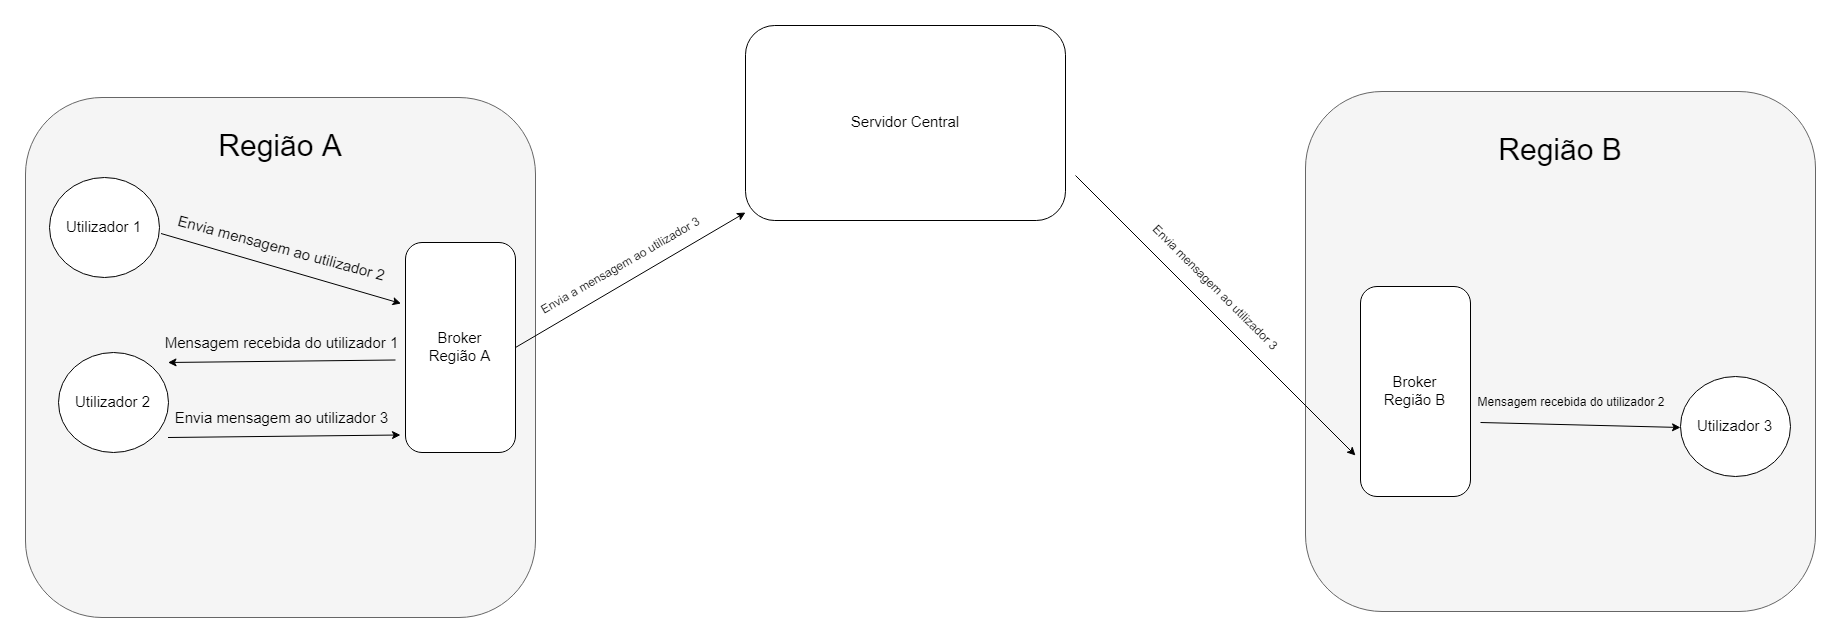
\includegraphics[width=1.3\textwidth]{./figures/diagram}
	}
\end{figure}

O utilizador é cliente do servidor regional. O servidor regional é servidor do utilizador e cliente do servidor central. O servidor central é servidor do servidor regional.

\section{Funcionamento}

Para puder utilizar o sistema, o utilizador deve escolher em qual região pretende-se conectar. Estando este conectado, é possível usufruir das seguintes funcionalidades:
\begin{itemize}
	\item Enviar mensagens para o utilizador;
	\item Criar grupos;
	\item Enviar mensagens para um grupo;
	\item Trocar de regiões;
	\item Sair de uma região.
\end{itemize}

\subsection{Funcionamento entre utilizadores}
Para um utilizador enviar uma mensagem para outro utilizador da mesma região o processo ocorre apenas no servidor dessa região. Caso o utilizador deseje enviar uma mensagem para outro utilizador fora da sua região, o servidor da região irá comunicar-se com o servidor central dizendo para este tratar de enviar a mensagem para um determinado utilizador que o servidor regional não tem conhecimento. O servidor central irá verificar em qual dos servidores regionais está presente o utilizador que tem de receber a mensagem e enviar a mensagem para esse servidor regional. Por sua vez, o servidor regional trata de entregar a mensagem ao utilizador.

\subsection{Funcionamento em grupo}
É possível ao utilizador criar grupos dentro de uma região e adicionar outros utilizadores quer estejam na mesma ou em diferentes regiões. Ao adicionar um utilizador de outra região, a informação desse grupo será replicada para essa região e para todas as outras regiões que contenham informação desse grupo. Apenas o criador do grupo tem permissão para eliminar esse grupo. Aos utilizadores que pertencem a um grupo, estes têm permissão para adicionar outros utilizadores. Os utilizadores que pertencem a um grupo nunca podem sair desse grupo, só sairão quando o criador apagar o grupo.